\tikzset{every picture/.style={line width=0.75pt}} %set default line width to 0.75pt

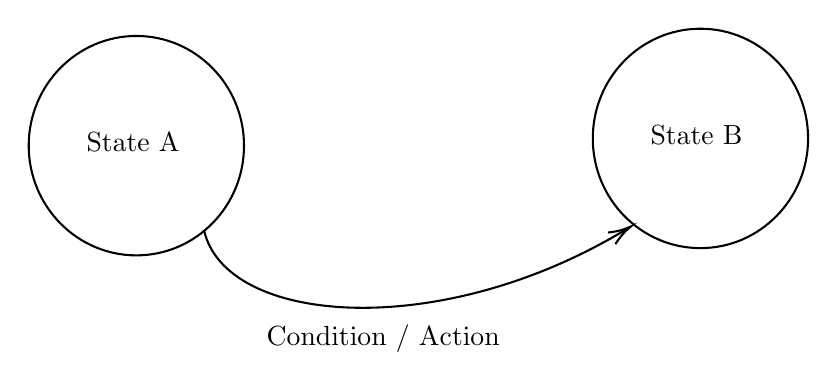
\begin{tikzpicture}[x=0.75pt,y=0.75pt,yscale=-1,xscale=1]
%uncomment if require: \path (0,777); %set diagram left start at 0, and has height of 777

%Shape: Ellipse [id:dp7032860404022366]
\draw   (10,63.35) .. controls (10,34.16) and (33.22,10.49) .. (61.87,10.49) .. controls (90.51,10.49) and (113.73,34.16) .. (113.73,63.35) .. controls (113.73,92.54) and (90.51,116.2) .. (61.87,116.2) .. controls (33.22,116.2) and (10,92.54) .. (10,63.35) -- cycle ;
%Shape: Ellipse [id:dp2228367254212833]
\draw   (281.77,59.85) .. controls (281.77,30.66) and (304.99,7) .. (333.63,7) .. controls (362.28,7) and (385.5,30.66) .. (385.5,59.85) .. controls (385.5,89.05) and (362.28,112.71) .. (333.63,112.71) .. controls (304.99,112.71) and (281.77,89.05) .. (281.77,59.85) -- cycle ;
%Curve Lines [id:da7146299088305332]
\draw    (94.44,103.97) .. controls (104.68,150.04) and (209.13,158.06) .. (298.85,103.06) ;
\draw [shift={(300.2,102.23)}, rotate = 508.15] [color={rgb, 255:red, 0; green, 0; blue, 0 }  ][line width=0.75]    (10.93,-3.29) .. controls (6.95,-1.4) and (3.31,-0.3) .. (0,0) .. controls (3.31,0.3) and (6.95,1.4) .. (10.93,3.29)   ;

% Text Node
\draw (36.37,55.72) node [anchor=north west][inner sep=0.75pt]   [align=left] {State A};
% Text Node
\draw (308.13,52.23) node [anchor=north west][inner sep=0.75pt]   [align=left] {State B};
% Text Node
\draw (123.18,148.33) node [anchor=north west][inner sep=0.75pt]   [align=left] {Condition / Action};
\end{tikzpicture}
